\documentclass[utf8x,hyperref={pdfpagelabels=false}]{beamer}

\usepackage[utf8x]{inputenc}
\usepackage[OT1]{fontenc}
\usepackage{amsmath,graphicx}
\usepackage{xcolor}
\usepackage{amsmath}
\usepackage{tikz}

\usetikzlibrary{arrows}
\usetikzlibrary{calc}

\usetheme{Malmoe}  % Now it's a beamer presentation with the lisa theme!        
\usecolortheme{beaver}
\setbeamertemplate{footline}[page number]
\setbeamertemplate{navigation symbols}{}

\title{Recurrent Neural Networks in Theano}

\author{%
Phil\'{e}mon Brakel
}
\date{August 11, 2015}

\definecolor{termblue}{RGB}{51, 51, 179}
\newcommand{\term}[1]{\textcolor{termblue}{#1}}

\begin{document}

\begin{frame}[plain]
 \titlepage
\end{frame}

\setcounter{page}{1}

\section{Recap RNNs}

\begin{frame}
\begin{figure}[t]
\centering
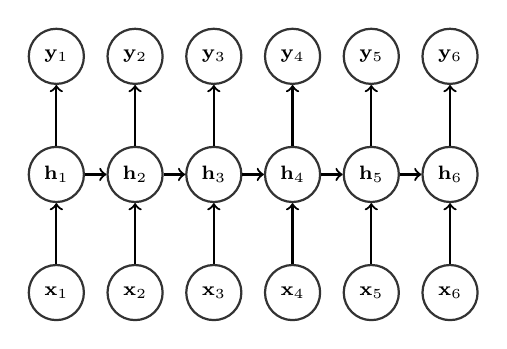
\begin{tikzpicture}[->,thick]
\scriptsize
\tikzstyle{main}=[circle, minimum size = 7mm, thick, draw =black!80, node distance = 12mm]
\foreach \name in {1,...,6}
    \node[main, fill = white!100] (y\name) at (\name,1.5) {$\mathbf{y}_\name$};
\foreach \name in {1,...,6}
    \node[main, fill = white!100] (h\name) at (\name,0) {$\mathbf{h}_\name$};
\foreach \name in {1,...,6}
    \node[main, fill = white!100] (x\name) at (\name,-1.5) {$\mathbf{x}_\name$};
\foreach \h in {1,...,6}
       {
        \path (x\h) edge (h\h);
        \path (h\h) edge (y\h);
       }
\foreach \current/\next in {1/2,2/3,3/4,4/5,5/6} 
       {
        \path (h\current) edge (h\next);
       }
    %\node[main] (G-\name) at (\x,0) {$\name$};
\end{tikzpicture}
\caption{Two Bidirectional Recurrent Neural Networks stacked on top of each
other.}
\label{fig:birnn}
\end{figure}
\end{frame}

\begin{frame}
\frametitle{Long Short-Term Memory}
\begin{figure}[t]
\centering
\includegraphics{lstmjozefowicz15}
\caption{LSTM\footnote{Taken from Jozefowicz et al. (2015)}}
\end{figure}
\end{frame}

\begin{frame}
\begin{figure}[t]
\centering
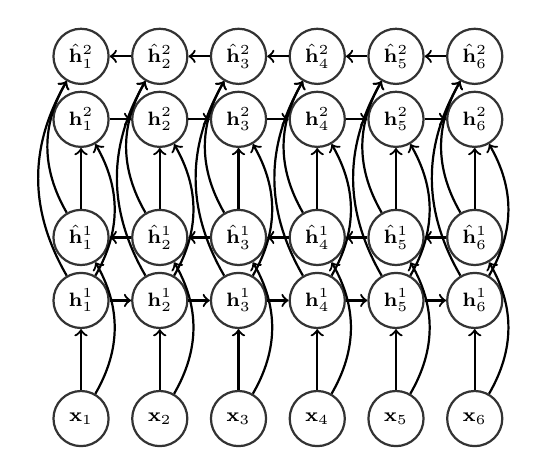
\begin{tikzpicture}[->,thick]
\scriptsize
\tikzstyle{main}=[circle, minimum size = 7mm, thick, draw =black!80, node distance = 12mm]
\foreach \name in {1,...,6}
    \node[main, fill = white!100] (l\name) at (\name,2.3) {$\mathbf{h}^2_\name$};
\foreach \name in {1,...,6}
    \node[main, fill = white!100] (k\name) at (\name,3.1) {$\hat{\mathbf{h}}^2_\name$};
\foreach \name in {1,...,6}
    \node[main, fill = white!100] (i\name) at (\name,.8) {$\hat{\mathbf{h}}^1_\name$};
\foreach \name in {1,...,6}
    \node[main, fill = white!100] (h\name) at (\name,0) {$\mathbf{h}^1_\name$};
\foreach \name in {1,...,6}
    \node[main, fill = white!100] (x\name) at (\name,-1.5) {$\mathbf{x}_\name$};
\foreach \h in {1,...,6}
       {
        \path (x\h) edge [bend right] (i\h);
        \path (x\h) edge (h\h);
        \path (i\h) edge [bend left] (k\h);
        \path (h\h) edge [bend right] (l\h);
        \path (h\h) edge [bend left] (k\h);
        \path (i\h) edge (l\h);
       }
\foreach \current/\next in {1/2,2/3,3/4,4/5,5/6} 
       {
        \path (i\next) edge (i\current);
        \path (h\current) edge (h\next);
        \path (k\next) edge (k\current);
        \path (l\current) edge (l\next);
       }
    %\node[main] (G-\name) at (\x,0) {$\name$};
\end{tikzpicture}
\caption{Two Bidirectional Recurrent Neural Networks stacked on top of each
other.}
\label{fig:birnn}
\end{figure}
\end{frame}

\begin{frame}

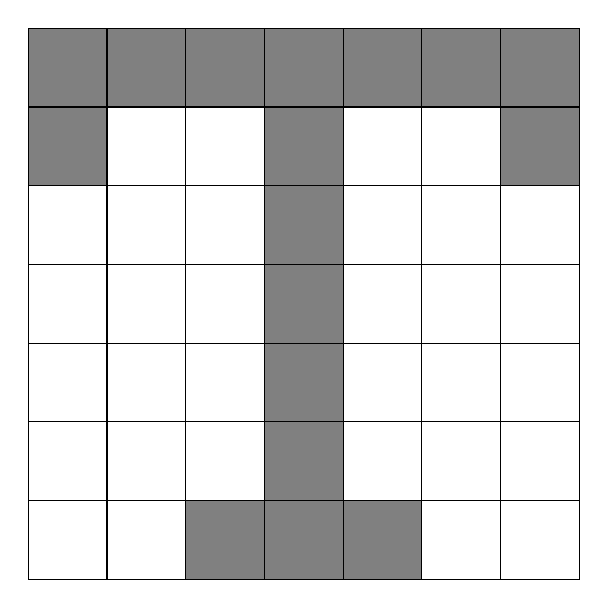
\begin{tikzpicture}
\tikzset{every cell/.style={draw=black}}
\tikzset{every cell 1/.style={fill=gray}}

   \foreach \row [count=\y] in {%
     {1,1,1,1,1,1,1},%
     {1,0,0,1,0,0,1},%
     {0,0,0,1,0,0,0},%
     {0,0,0,1,0,0,0},%
     {0,0,0,1,0,0,0},%
     {0,0,0,1,0,0,0},%
     {0,0,1,1,1,0,0}}
     \foreach \cell [count=\x] in \row  
        \path [every cell/.try, every cell \cell/.try]
           (\x,-\y) rectangle ++(1,1);
\end{tikzpicture}
\end{frame}

\section{RNNs with scan}




\end{document}
